% !TeX root = ../handout.tex

\section{Einleitung und Motivation}

Seit über 40 Jahren ist das Konzept des \emph{Data Sharing} Bestandteil der Forschung.
Data Sharing beschreibt den Prozess, bei dem Dritten Zugriff auf Daten gewährt wird, auf die sie sonst keinen Zugriff hätten (vgl. Beispiel in \autoref{fig:example-data-donation}).
Das Internet und die Einführung von Smartphones ermöglicht es, nahezu sofort Daten zu erhalten und weiterzuverteilen.
Auch im betrieblichen Kontext sind Daten essenziell.
Sie sind für nahezu alle Geschäftsprozesse notwendig, sodass sie sich vom \enquote{Nebenprodukt} zur strategischen Ressource entwickelten~\cite{mollerIndustrialDataEcosystems2024}.
Es gibt viele Bedenken beim Teilen von Daten, wie bspw. der Angst vor unberechtigter Weitergabe, Missbrauch von Daten oder Kontrollverlust~\cite{mollerIndustrialDataEcosystems2024}.
Für ein multilaterales Datennetz fehlt Vertrauen.

\begin{figure}
    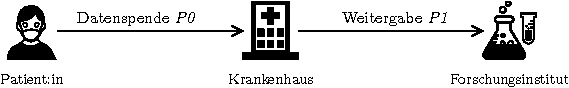
\includegraphics[width=\textwidth]{./assets/example_horizontal.drawio.pdf}
    \caption{Beispiel für Data Sharing: Datenspende zur Weiterverwendung für Forschung}
    \label{fig:example-data-donation}
\end{figure}

Um Daten zwischen verschiedenen Akteuren zu teilen, ist oft eine Datenintegration, bspw. via \emph{Extract, Transform, Load} (ETL) notwendig, welche essenziell für den Erfolg von Geschäftsprozessen ist.
Solche Integrationen sind oftmals aufwendig und zeitintensiv.
Nach Abschluss haben sich die Modelle und Projekte teilweise schon wieder verändert, sodass Inkonsistenzen und hohe Kosten durch die wiederholte Ausführung von Schritten entstehen.
Durch die Kostenintensitivität liegt die Einstiegsbarriere für neue Akteure hoch, wodurch Zugänglichkeit und Innovationsfähigkeit eingeschränkt werden.
Ein effizientes, schnelles und günstiges Verfahren, bei denen Daten stets verfügbar, konsistent und zugänglich sind, ist anzustreben.

Da Daten als wertvolles Wirtschaftsgut zu betrachten sind, werden diese \emph{en masse} gespeichert.
Da Nutzende ihre Daten und Privatsphäre oft nicht kontrollieren können, werden diese nur zurückhaltend geteilt.
Aufgrund von mangelndem Vertrauen und dadurch mangelnder Kooperation, werden dieselben Daten mehrfach an verschiedenen Orten gespeichert.
Somit entstehen große Datensilos, welche inkonsistente und teils veraltete Daten enthalten.
Wünschenswert wäre die Verfügbarkeit von aktuellen, konsistenten Daten mit garantierter Datensouveränität.

An dieser Stelle setzt das Konzept der \emph{Data Spaces} an. Dieses adressiert die Probleme, in dem es einen multilateralen, sicheren und vertrauenswürdigen Datenaustausch anstrebt, welches Datensouveränität garantiert~\cite{mollerIndustrialDataEcosystems2024}.
Der Begründer des \emph{World Wide Web}s, Tim Berners"=Lee, stellte dazu 2016 den Solid"=Standard (ehem. \emph{Social Linked Data}) vor, welches ein Fundament für offene, dezentralisierte Netzwerke für einen souveränen Datenaustausch ermöglichen möchte~\cite{mecklerWebLinkedData2023}.
